\documentclass[11pt]{article}
\usepackage{amsmath,amssymb,amsfonts}
\usepackage{graphicx, float}
\usepackage{pgfplots}
\usepackage{multicol}
\usepackage{enumitem}
\usepgfplotslibrary{fillbetween}
\pgfplotsset{compat=1.16,width=10cm}


\setlength{\topmargin}{-.5in} \setlength{\textheight}{9.25in}
\setlength{\oddsidemargin}{0in} \setlength{\textwidth}{6.8in}


\begin{document}

\Large

\noindent{\bf Name: \hfill Date: \hfill Exam 3 \hfill Precalculus - Hargus}
\medskip\hrule
\vspace{10pt}

\noindent \textbf{Instructions:} Please \textbf{show all work} (partial credit will be given for correct work, even if your answer is wrong). You may use a calculator.

\begin{enumerate}

\item (10 points) True or false? (circle your answer)
\begin{enumerate}[itemsep=20pt, label={\alph*)}]
\item Each term in a geometric sequence is the previous term plus some constant.  \\ \null\hfill \textbf{T} or \textbf{F}
\item A proof by induction requires an ``anchor'' and an ``inductive step''.\\ \null\hfill \textbf{T} or \textbf{F}
\item The sequence with $a_1 = 5$ and $a_{k+1} = a_k - 1$ converges. \null\hfill \textbf{T} or \textbf{F}

\item The series $\sum_{k=1}^{\infty} 2^k$ converges. \null\hfill \textbf{T} or \textbf{F}
\item The series $\frac{1}{2}+ \frac{1}{4}+ \frac{1}{8}+...$ converges. \null\hfill \textbf{T} or \textbf{F}
\end{enumerate}

\vspace{20pt}
\item (4 points) Compute the sum $\sum_{k=1}^{200} 6k+4$. (Hint: note that this is an arithmetic series)

\vspace{120pt}
\begin{flushright}
$\sum_{k=1}^{50} 6k+4 = \rule{3cm}{0.4pt}$
\end{flushright}

\newpage

\item (8 points) Simplify the expression to either 1 or -1.

\begin{enumerate}[itemsep=80pt, label={\alph*)}]
    \item $\displaystyle \cos(-x) \sec(x) $
    \item $\displaystyle \frac{\sin^2(x)-1}{\cos^2x} $
\end{enumerate}

\vspace{120pt}

\item (8 points) Prove the identity.
\begin{enumerate}[itemsep=140pt, label={\alph*)}]
    \item $\displaystyle (\sin x)(\cot x + \cos x \tan x) = \cos x + \sin^2 x$
    \item $\displaystyle (1-2\cos^2 x + \cos^4 x)(\sin x) = \sin^5 x$
\end{enumerate}

\newpage

\item (6 points) Use a half-angle identity to find the exact value of $\sin(75^{\circ})$. Show your work.
\vspace{100pt}
\begin{flushright}
$\sin(75^{\circ})= \rule{3cm}{0.4pt}$
\end{flushright}
\vspace{20pt}

\item (6 points) Find all solutions to the equation $\cos(2x) = \cos(x)$ in the interval $[0,2\pi )$.
\vspace{100pt}
\begin{flushright}
$x= \rule{3cm}{0.4pt}$
\end{flushright}
\vspace{20pt}


\item (12 points) Find an \textbf{explicit} rule for the $n$th term of the sequence.
\begin{enumerate}[itemsep=30pt, label={\alph*)}]
\item $4, 2, 0, -2, ...$
\begin{flushright}
$a_n$= $\rule{3cm}{0.4pt}$
\end{flushright}
\item $3, 1, \frac{1}{3}, ...$
\begin{flushright}
$a_n$= $\rule{3cm}{0.4pt}$
\end{flushright}
\item $a_1 = 5$, $a_n$ = $6 \cdot a_{n-1}$
\begin{flushright}
$a_n$= $\rule{3cm}{0.4pt}$
\end{flushright}
\end{enumerate}

\newpage

\item (15 points)
\begin{enumerate}[itemsep=60pt, label={\alph*)}]
\item Connor has 12 pairs of socks and 3 pairs of shoes. How many ways are there for him to choose a set of socks and shoes to wear?
\begin{flushright}
Ways: $\rule{3cm}{0.4pt}$
\end{flushright}
\item If the classroom has 9 chairs and there are 9 students, how many ways are there to choose who sits in each chair?
\begin{flushright}
Ways: $\rule{3cm}{0.4pt}$
\end{flushright}
\item If the classroom has 9 chairs and there are 9 students, how many ways are there to choose who sits in each chair if Chester needs to be in the back row?
\begin{flushright}
Ways: $\rule{3cm}{0.4pt}$
\end{flushright}
\item If we roll two six-sided dice, what is the probability that the sum of the dice is 11?
\begin{flushright}
Probability: $\rule{3cm}{0.4pt}$
\end{flushright}
\item When it rains, Steven never plays basketball. If it does not rain, Steven plays basketball 50\% of the time. If there is a 60\% chance of rain tomorrow, what is the probability that Steven will play basketball?
\begin{flushright}
Probability: $\rule{3cm}{0.4pt}$
\end{flushright}
\end{enumerate}

\newpage

\item (15 points) Solve for missing sides and angles using the Law of Cosines and Law of Sines.

(a) \\

\tikzset{every picture/.style={line width=0.75pt}} %set default line width to 0.75pt        

\begin{tikzpicture}[x=0.75pt,y=0.75pt,yscale=-1,xscale=1]
%uncomment if require: \path (0,300); %set diagram left start at 0, and has height of 300

%Shape: Triangle [id:dp610907045225627] 
\draw   (179.27,52.14) -- (303.7,109.67) -- (80.93,109.67) -- cycle ;

% Text Node
\draw (171.47,28.1) node [anchor=north west][inner sep=0.75pt]    {$A$};
% Text Node
\draw (55.69,100.7) node [anchor=north west][inner sep=0.75pt]    {$B$};
% Text Node
\draw (314.07,100.7) node [anchor=north west][inner sep=0.75pt]    {$C$};
% Text Node
\draw (162.59,66.45) node [anchor=north west][inner sep=0.75pt]    {$115^\circ$};
% Text Node
\draw (235.25,56.87) node [anchor=north west][inner sep=0.75pt]    {$22$};
% Text Node
\draw (114.86,59.61) node [anchor=north west][inner sep=0.75pt]    {$17$};


\end{tikzpicture}

\begin{flushright}
$a=\rule{3cm}{0.4pt}$
\end{flushright}
\begin{flushright}
$\angle B=\rule{3cm}{0.4pt}$
\end{flushright}
\begin{flushright}
$\angle C=\rule{3cm}{0.4pt}$
\end{flushright}
\vspace{40pt}



(b) \\

\tikzset{every picture/.style={line width=0.75pt}} %set default line width to 0.75pt        

\begin{tikzpicture}[x=0.75pt,y=0.75pt,yscale=-1,xscale=1]
%uncomment if require: \path (0,300); %set diagram left start at 0, and has height of 300

%Shape: Triangle [id:dp7075641536091434] 
\draw   (173.26,61.8) -- (399.49,160.79) -- (129.01,160.79) -- cycle ;

% Text Node
\draw (165.47,34.18) node [anchor=north west][inner sep=0.75pt]    {$E$};
% Text Node
\draw (104.69,155.32) node [anchor=north west][inner sep=0.75pt]    {$D$};
% Text Node
\draw (410.07,151.39) node [anchor=north west][inner sep=0.75pt]    {$F$};
% Text Node
\draw (170.59,78.12) node [anchor=north west][inner sep=0.75pt]    {$89^{\circ }$};
% Text Node
\draw (143.25,134.68) node [anchor=north west][inner sep=0.75pt]    {$59^{\circ }$};
% Text Node
\draw (130.86,89.79) node [anchor=north west][inner sep=0.75pt]    {$14$};


\end{tikzpicture}



\begin{flushright}
$d=\rule{3cm}{0.4pt}$
\end{flushright}
\begin{flushright}
$e=\rule{3cm}{0.4pt}$
\end{flushright}
\begin{flushright}
$\angle F=\rule{3cm}{0.4pt}$
\end{flushright}
\vspace{20pt}

\newpage

(c) \\

\tikzset{every picture/.style={line width=0.75pt}} %set default line width to 0.75pt        

\begin{tikzpicture}[x=0.75pt,y=0.75pt,yscale=-1,xscale=1]
%uncomment if require: \path (0,300); %set diagram left start at 0, and has height of 300

%Shape: Triangle [id:dp6565210684786356] 
\draw   (217.98,49.15) -- (235.2,203.12) -- (85.63,203.12) -- cycle ;

% Text Node
\draw (211.8,22.42) node [anchor=north west][inner sep=0.75pt]    {$H$};
% Text Node
\draw (64.49,198.84) node [anchor=north west][inner sep=0.75pt]    {$G$};
% Text Node
\draw (249.31,198.74) node [anchor=north west][inner sep=0.75pt]    {$I$};
% Text Node
\draw (192.61,75.32) node [anchor=north west][inner sep=0.75pt]    {$39^{\circ }$};
% Text Node
\draw (104.85,180.29) node [anchor=north west][inner sep=0.75pt]    {$67^{\circ }$};
% Text Node
\draw (236.5,118.91) node [anchor=north west][inner sep=0.75pt]    {$6$};

\end{tikzpicture}

\begin{flushright}
$h=\rule{3cm}{0.4pt}$
\end{flushright}
\begin{flushright}
$i=\rule{3cm}{0.4pt}$
\end{flushright}
\begin{flushright}
$\angle I=\rule{3cm}{0.4pt}$
\end{flushright}
\vspace{40pt}


\item (4 points) How many triangles can be made with the measurements $B=30^{\circ}$, $b=5$, $c=8$? (with angle $B$ opposite from side $b$) 
\vspace{100pt}
\begin{flushright}
Number of triangles: $\rule{3cm}{0.4pt}$
\end{flushright}

\newpage

\item (4 points) What is the area of the triangle with measurements $A=50^{\circ}$, $b=10$, $c=6$?
\vspace{100pt}
\begin{flushright}
Area $= \rule{3cm}{0.4pt}$
\end{flushright}
\vspace{20pt}

\item (\textbf{Extra Credit:} 5 points) Prove the following statement for all positive integers $n$ using induction. \\
$$1 + 2 + 4 + ... + 2^{n-1} = 2^n - 1 $$

\end{enumerate}

\end{document} 